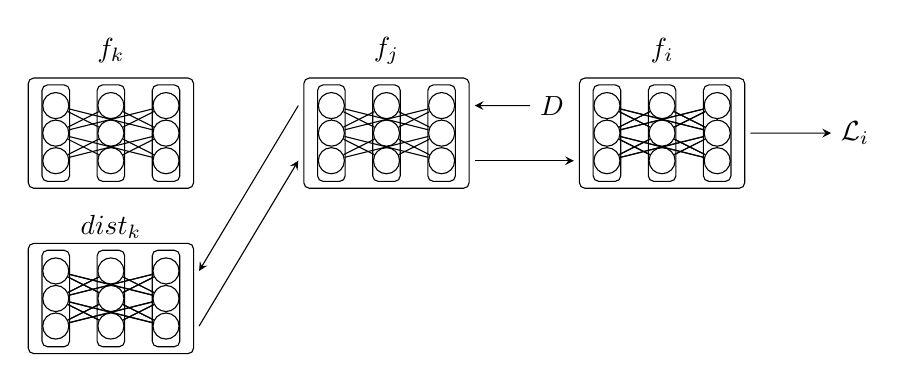
\begin{tikzpicture}


\begin{scope}[scale=0.7]

    \node[] at (1,2) {$f_j$};
    \node[] at (-4,2) {$f_k$};
    \node[] at (6,2) {$f_i$};
    
    \node[] at (-4,-1.2) {$\text{dist}_k$};

    

    %\draw[-stealth] (-7,3) node[below] {$\mathbf{M_1}$} -- (-5.5, 0.5);
    %\draw[-stealth] (-2.5, 0.5) -- (-1.5, 1.75) node[above] {$\mathcal{L}_k$};
    %\draw[-stealth] (2.5, 0.5) -- (3.5, 1.75) node[above] {$\mathcal{L}_j$};
    
    \node[] (m) at (4, 1) {$D$};
    \node[] (l) at (9.5, 0.5) {$\mathcal{L}_i$};
    
    \draw[-stealth] (m) -- (2.6, 1);
    \draw[-stealth] (7.6, 0.5) -- (l);

    
   % \draw[-stealth] (7.5, 0.5) -- (8.5, 1.75) node[above] {$\mathcal{L}_i$};
    
    \draw[-stealth] (2.6, 0) -- (4.4, 0);
    \draw[-stealth] (-0.6, 1) -- (-2.4, -2.0);
    \draw[-stealth] (-2.4, -3) -- (-0.6, 0);
    

    \foreach \x in {0,...,2}
        {
        \foreach \y in {0,...,2} 
            {
            \node[circle, draw, scale=1] (\x\y) at (\x, \y * 0.5) {};
            }
        \draw[rounded corners=2] (\x - 0.25, 1.375) rectangle ++(0.5, -1.75);
        }
    \draw[rounded corners=2] (-0.5, -0.5) rectangle ++(3, 2);
    
    
    \foreach \x in {0,...,2}
        {
        \foreach \y in {1,2}
            {
            \pgfmathsetmacro\yi{int(\y - 1)}
            \draw (\x\yi)edge(0\y);
            \draw (\x\yi)edge(1\y);
            \draw (\x\yi)edge(2\y);
            }
        }
        
     \foreach \x in {0,...,2}
        {
        \foreach \y in {0,...,2} 
            {
            \node[circle, draw, scale=1] (\x\y) at (\x - 5, \y * 0.5) {};
            }
        \draw[rounded corners=2] (\x - 0.25 - 5, 1.375) rectangle ++(0.5, -1.75);
        }
    \draw[rounded corners=2] (-0.5 - 5, -0.5) rectangle ++(3, 2);

    
    \foreach \x in {0,...,2}
        {
        \foreach \y in {1,2}
            {
            \pgfmathsetmacro\yi{int(\y - 1)}
            \draw (\x\yi)edge(0\y);
            \draw (\x\yi)edge(1\y);
            \draw (\x\yi)edge(2\y);
            }
        }
        
    \foreach \x in {0,...,2}
        {
        \foreach \y in {0,...,2} 
            {
            \node[circle, draw, scale=1] (\x\y) at (\x + 5, \y * 0.5) {};
            }
        \draw[rounded corners=2] (\x - 0.25 + 5, 1.375) rectangle ++(0.5, -1.75);
        }
    \draw[rounded corners=2] (-0.5 + 5, -0.5) rectangle ++(3, 2);

    
    \foreach \x in {0,...,2}
        {
        \foreach \y in {1,2}
            {
            \pgfmathsetmacro\yi{int(\y - 1)}
            \draw (\x\yi)edge(0\y);
            \draw (\x\yi)edge(1\y);
            \draw (\x\yi)edge(2\y);
            }
        }
        
        
    %  \foreach \x in {0,...,2}
    %     {
    %     \foreach \y in {0,...,2} 
    %         {
    %         \node[circle, draw, scale=1] (\x\y) at (\x, \y * 0.5 - 4) {};
    %         }
    %     \draw[rounded corners=2] (\x - 0.25, 1.375 - 4) rectangle ++(0.5, -1.75);
    %     }
    % \draw[rounded corners=2] (-0.5, -0.5 - 4) rectangle ++(3, 2);

    
    \foreach \x in {0,...,2}
        {
        \foreach \y in {1,2}
            {
            \pgfmathsetmacro\yi{int(\y - 1)}
            \draw (\x\yi)edge(0\y);
            \draw (\x\yi)edge(1\y);
            \draw (\x\yi)edge(2\y);
            }
        }
        
     \foreach \x in {0,...,2}
        {
        \foreach \y in {0,...,2} 
            {
            \node[circle, draw, scale=1] (\x\y) at (\x - 5, \y * 0.5 - 3) {};
            }
        \draw[rounded corners=2] (\x - 0.25 - 5, 1.375 - 3) rectangle ++(0.5, -1.75);
        }
    \draw[rounded corners=2] (-0.5 - 5, -0.5- 3) rectangle ++(3, 2);

    
    \foreach \x in {0,...,2}
        {
        \foreach \y in {1,2}
            {
            \pgfmathsetmacro\yi{int(\y - 1)}
            \draw (\x\yi)edge(0\y);
            \draw (\x\yi)edge(1\y);
            \draw (\x\yi)edge(2\y);
            }
        }
        
    %  \foreach \x in {0,...,2}
    %     {
    %     \foreach \y in {0,...,2} 
    %         {
    %         \node[circle, draw, scale=1] (\x\y) at (\x + 5, \y * 0.5 - 4) {};
    %         }
    %     \draw[rounded corners=2] (\x - 0.25 + 5, 1.375 - 4) rectangle ++(0.5, -1.75);
    %     }
    % \draw[rounded corners=2] (-0.5 + 5, -0.5- 4) rectangle ++(3, 2);

    
    \foreach \x in {0,...,2}
        {
        \foreach \y in {1,2}
            {
            \pgfmathsetmacro\yi{int(\y - 1)}
            \draw (\x\yi)edge(0\y);
            \draw (\x\yi)edge(1\y);
            \draw (\x\yi)edge(2\y);
            }
        }
        
 
    
    
    % \foreach \y in {0,...,2}
    %     {
    %     \foreach \x in {0,...,2} 
    %         {
    %         \pgfmathsetmacro\xi{(6 + \x*0.5)}
    %         \node[circle, draw] (\x\y) at (\xi,\y) {};
    %         }
    %     \draw[rounded corners=2] (6 + -0.375,\y+0.25) rectangle ++(1.75,-0.5);
    %     }
    % \draw[rounded corners=2] (6 + -0.5, -0.4) rectangle ++(2, 2.8);

    
    % \foreach \x in {0,...,2}
    %     {
    %     \foreach \y in {1,2}
    %         {
    %         \pgfmathsetmacro\yi{int(\y - 1)}
    %         \draw (\x\yi)edge(0\y);
    %         \draw (\x\yi)edge(1\y);
    %         \draw (\x\yi)edge(2\y);
    %         }
    %     }
        
    % \draw[-stealth] (6 + 0.5,-1) node[below] {$\mathbf{M_1}$} -- (6 + 0.5,-0.5);
    % \draw[-stealth] (6 + 0.5,2.5) -- (6 + 0.5,3) node[above] {$\mathcal{L}_1$};
    
    
    % \foreach \y in {0,...,2}
    %     {
    %     \foreach \x in {0,...,2} 
    %         {
    %         \pgfmathsetmacro\xi{(6 + \x*0.5)}
    %         \node[circle, draw] (\x\y) at (\xi,-6 +  \y) {};
    %         }
    %     \draw[rounded corners=2] (6 + -0.375, -6 + \y+0.25) rectangle ++(1.75,-0.5);
    %     }
    % \draw[rounded corners=2] (6 + -0.5, -6 + -0.4) rectangle ++(2, 2.8);

    
    % \foreach \x in {0,...,2}
    %     {
    %     \foreach \y in {1,2}
    %         {
    %         \pgfmathsetmacro\yi{int(\y - 1)}
    %         \draw (\x\yi)edge(0\y);
    %         \draw (\x\yi)edge(1\y);
    %         \draw (\x\yi)edge(2\y);
    %         }
    %     }
        
    % \draw[-stealth] (6 + 0.5, -6 + -1) node[below] {$\mathbf{M_2}$} -- (6 + 0.5, -6 +  -0.5);
    % \draw[-stealth] (6 + 0.5, -6 + 2.5) -- (6 + 0.5, -6 + 3) node[above] {$\mathcal{L}_2$};
    
    
    %  \foreach \y in {0,...,2}
    %     {
    %     \foreach \x in {0,...,2} 
    %         {
    %         \pgfmathsetmacro\xi{(12 + \x*0.5)}
    %         \node[circle, draw] (\x\y) at (\xi, -6 +  \y) {};
    %         }
    %     \draw[rounded corners=2] (12 + -0.375, -6 + \y+0.25) rectangle ++(1.75,-0.5);
    %     }
    % \draw[rounded corners=2] (12 + -0.5, -6 + -0.4) rectangle ++(2, 2.8);

    
    % \foreach \x in {0,...,2}
    %     {
    %     \foreach \y in {1,2}
    %         {
    %         \pgfmathsetmacro\yi{int(\y - 1)}
    %         \draw (\x\yi)edge(0\y);
    %         \draw (\x\yi)edge(1\y);
    %         \draw (\x\yi)edge(2\y);
    %         }
    %     }
        
    % \draw[-stealth] (12 + 0.5, -6 + -1) node[below] {$\mathbf{M_3}$} -- (12 + 0.5, -6 +  -0.5);
    % \draw[-stealth] (12 + 0.5, -6 + 2.5) -- (12 + 0.5, -6 + 3) node[above] {$\mathcal{L}_3$};
    
    
    % \draw[-stealth] (5, 1) -- (2, 1);
    % \draw[-stealth] (5, -5) -- (2, -1);
    % \draw[-stealth] (11, -5) -- (8, -1);
    % \draw[-stealth] (11, -5) -- (8, -5);
    
    % \node[] at (-1,2) {$f_0$};
    % \node[] at (5,2) {$f_1$};
    % \node[] at (5,-4) {$f_2$};
    % \node[] at (11,-4) {$f_3$};

    
\end{scope}


\end{tikzpicture}